% Options for packages loaded elsewhere
\PassOptionsToPackage{unicode}{hyperref}
\PassOptionsToPackage{hyphens}{url}
%
\documentclass[
]{article}
\title{2021 4th}
\author{}
\date{\vspace{-2.5em}}

\usepackage{amsmath,amssymb}
\usepackage{lmodern}
\usepackage{iftex}
\ifPDFTeX
  \usepackage[T1]{fontenc}
  \usepackage[utf8]{inputenc}
  \usepackage{textcomp} % provide euro and other symbols
\else % if luatex or xetex
  \usepackage{unicode-math}
  \defaultfontfeatures{Scale=MatchLowercase}
  \defaultfontfeatures[\rmfamily]{Ligatures=TeX,Scale=1}
\fi
% Use upquote if available, for straight quotes in verbatim environments
\IfFileExists{upquote.sty}{\usepackage{upquote}}{}
\IfFileExists{microtype.sty}{% use microtype if available
  \usepackage[]{microtype}
  \UseMicrotypeSet[protrusion]{basicmath} % disable protrusion for tt fonts
}{}
\makeatletter
\@ifundefined{KOMAClassName}{% if non-KOMA class
  \IfFileExists{parskip.sty}{%
    \usepackage{parskip}
  }{% else
    \setlength{\parindent}{0pt}
    \setlength{\parskip}{6pt plus 2pt minus 1pt}}
}{% if KOMA class
  \KOMAoptions{parskip=half}}
\makeatother
\usepackage{xcolor}
\IfFileExists{xurl.sty}{\usepackage{xurl}}{} % add URL line breaks if available
\IfFileExists{bookmark.sty}{\usepackage{bookmark}}{\usepackage{hyperref}}
\hypersetup{
  pdftitle={2021 4th},
  hidelinks,
  pdfcreator={LaTeX via pandoc}}
\urlstyle{same} % disable monospaced font for URLs
\usepackage[margin=1in]{geometry}
\usepackage{color}
\usepackage{fancyvrb}
\newcommand{\VerbBar}{|}
\newcommand{\VERB}{\Verb[commandchars=\\\{\}]}
\DefineVerbatimEnvironment{Highlighting}{Verbatim}{commandchars=\\\{\}}
% Add ',fontsize=\small' for more characters per line
\usepackage{framed}
\definecolor{shadecolor}{RGB}{248,248,248}
\newenvironment{Shaded}{\begin{snugshade}}{\end{snugshade}}
\newcommand{\AlertTok}[1]{\textcolor[rgb]{0.94,0.16,0.16}{#1}}
\newcommand{\AnnotationTok}[1]{\textcolor[rgb]{0.56,0.35,0.01}{\textbf{\textit{#1}}}}
\newcommand{\AttributeTok}[1]{\textcolor[rgb]{0.77,0.63,0.00}{#1}}
\newcommand{\BaseNTok}[1]{\textcolor[rgb]{0.00,0.00,0.81}{#1}}
\newcommand{\BuiltInTok}[1]{#1}
\newcommand{\CharTok}[1]{\textcolor[rgb]{0.31,0.60,0.02}{#1}}
\newcommand{\CommentTok}[1]{\textcolor[rgb]{0.56,0.35,0.01}{\textit{#1}}}
\newcommand{\CommentVarTok}[1]{\textcolor[rgb]{0.56,0.35,0.01}{\textbf{\textit{#1}}}}
\newcommand{\ConstantTok}[1]{\textcolor[rgb]{0.00,0.00,0.00}{#1}}
\newcommand{\ControlFlowTok}[1]{\textcolor[rgb]{0.13,0.29,0.53}{\textbf{#1}}}
\newcommand{\DataTypeTok}[1]{\textcolor[rgb]{0.13,0.29,0.53}{#1}}
\newcommand{\DecValTok}[1]{\textcolor[rgb]{0.00,0.00,0.81}{#1}}
\newcommand{\DocumentationTok}[1]{\textcolor[rgb]{0.56,0.35,0.01}{\textbf{\textit{#1}}}}
\newcommand{\ErrorTok}[1]{\textcolor[rgb]{0.64,0.00,0.00}{\textbf{#1}}}
\newcommand{\ExtensionTok}[1]{#1}
\newcommand{\FloatTok}[1]{\textcolor[rgb]{0.00,0.00,0.81}{#1}}
\newcommand{\FunctionTok}[1]{\textcolor[rgb]{0.00,0.00,0.00}{#1}}
\newcommand{\ImportTok}[1]{#1}
\newcommand{\InformationTok}[1]{\textcolor[rgb]{0.56,0.35,0.01}{\textbf{\textit{#1}}}}
\newcommand{\KeywordTok}[1]{\textcolor[rgb]{0.13,0.29,0.53}{\textbf{#1}}}
\newcommand{\NormalTok}[1]{#1}
\newcommand{\OperatorTok}[1]{\textcolor[rgb]{0.81,0.36,0.00}{\textbf{#1}}}
\newcommand{\OtherTok}[1]{\textcolor[rgb]{0.56,0.35,0.01}{#1}}
\newcommand{\PreprocessorTok}[1]{\textcolor[rgb]{0.56,0.35,0.01}{\textit{#1}}}
\newcommand{\RegionMarkerTok}[1]{#1}
\newcommand{\SpecialCharTok}[1]{\textcolor[rgb]{0.00,0.00,0.00}{#1}}
\newcommand{\SpecialStringTok}[1]{\textcolor[rgb]{0.31,0.60,0.02}{#1}}
\newcommand{\StringTok}[1]{\textcolor[rgb]{0.31,0.60,0.02}{#1}}
\newcommand{\VariableTok}[1]{\textcolor[rgb]{0.00,0.00,0.00}{#1}}
\newcommand{\VerbatimStringTok}[1]{\textcolor[rgb]{0.31,0.60,0.02}{#1}}
\newcommand{\WarningTok}[1]{\textcolor[rgb]{0.56,0.35,0.01}{\textbf{\textit{#1}}}}
\usepackage{graphicx}
\makeatletter
\def\maxwidth{\ifdim\Gin@nat@width>\linewidth\linewidth\else\Gin@nat@width\fi}
\def\maxheight{\ifdim\Gin@nat@height>\textheight\textheight\else\Gin@nat@height\fi}
\makeatother
% Scale images if necessary, so that they will not overflow the page
% margins by default, and it is still possible to overwrite the defaults
% using explicit options in \includegraphics[width, height, ...]{}
\setkeys{Gin}{width=\maxwidth,height=\maxheight,keepaspectratio}
% Set default figure placement to htbp
\makeatletter
\def\fps@figure{htbp}
\makeatother
\setlength{\emergencystretch}{3em} % prevent overfull lines
\providecommand{\tightlist}{%
  \setlength{\itemsep}{0pt}\setlength{\parskip}{0pt}}
\setcounter{secnumdepth}{-\maxdimen} % remove section numbering
\ifLuaTeX
  \usepackage{selnolig}  % disable illegal ligatures
\fi

\begin{document}
\maketitle

\hypertarget{fourth-session}{%
\section{Fourth session}\label{fourth-session}}

compare gapminder wide vs long

gap\_wide \textless-
read\_csv(``\href{https://bit.ly/gapminder-rsu\%22}{https://bit.ly/gapminder-rsu'')})

Load the packages

\begin{Shaded}
\begin{Highlighting}[]
\NormalTok{pacman}\SpecialCharTok{::}\FunctionTok{p\_load}\NormalTok{(tidyverse, }\CommentTok{\# several datascience packages}
\NormalTok{               palmerpenguins, }\CommentTok{\# data}
\NormalTok{               gapminder, }\CommentTok{\#data,}
\NormalTok{               gtsummary) }\CommentTok{\# for tables) }
\end{Highlighting}
\end{Shaded}

\begin{Shaded}
\begin{Highlighting}[]
\NormalTok{gap\_wide }\OtherTok{\textless{}{-}} \FunctionTok{read\_csv}\NormalTok{(}\StringTok{"https://bit.ly/gapminder{-}rsu"}\NormalTok{)}
\end{Highlighting}
\end{Shaded}

\begin{verbatim}
## Rows: 142 Columns: 38
\end{verbatim}

\begin{verbatim}
## -- Column specification --------------------------------------------------------
## Delimiter: ","
## chr  (2): continent, country
## dbl (36): gdpPercap_1952, gdpPercap_1957, gdpPercap_1962, gdpPercap_1967, gd...
\end{verbatim}

\begin{verbatim}
## 
## i Use `spec()` to retrieve the full column specification for this data.
## i Specify the column types or set `show_col_types = FALSE` to quiet this message.
\end{verbatim}

\hypertarget{data-basics}{%
\subsection{Data basics}\label{data-basics}}

\hypertarget{filtering}{%
\paragraph{Filtering}\label{filtering}}

Filter by species == Adelie

\includegraphics{https://d33wubrfki0l68.cloudfront.net/b58f5f2b6a73f15e90a3c6bf8db8ba67a1ca365b/020d8/images/cheatsheets/filter.png}

\begin{Shaded}
\begin{Highlighting}[]
\NormalTok{penguins }\SpecialCharTok{\%\textgreater{}\%} 
  \FunctionTok{filter}\NormalTok{(species }\SpecialCharTok{==} \StringTok{"Adelie"}\NormalTok{)}
\end{Highlighting}
\end{Shaded}

\begin{verbatim}
## # A tibble: 152 x 8
##    species island    bill_length_mm bill_depth_mm flipper_length_mm body_mass_g
##    <fct>   <fct>              <dbl>         <dbl>             <int>       <int>
##  1 Adelie  Torgersen           39.1          18.7               181        3750
##  2 Adelie  Torgersen           39.5          17.4               186        3800
##  3 Adelie  Torgersen           40.3          18                 195        3250
##  4 Adelie  Torgersen           NA            NA                  NA          NA
##  5 Adelie  Torgersen           36.7          19.3               193        3450
##  6 Adelie  Torgersen           39.3          20.6               190        3650
##  7 Adelie  Torgersen           38.9          17.8               181        3625
##  8 Adelie  Torgersen           39.2          19.6               195        4675
##  9 Adelie  Torgersen           34.1          18.1               193        3475
## 10 Adelie  Torgersen           42            20.2               190        4250
## # ... with 142 more rows, and 2 more variables: sex <fct>, year <int>
\end{verbatim}

Filter by two conditions Adelie \& island == Dream

Filter body\_mass\_g \textless{} 3000

\begin{Shaded}
\begin{Highlighting}[]
\NormalTok{penguins }\SpecialCharTok{\%\textgreater{}\%} 
  \FunctionTok{filter}\NormalTok{(species }\SpecialCharTok{==} \StringTok{"Adelie"} \SpecialCharTok{\&}\NormalTok{ island }\SpecialCharTok{!=} \StringTok{"Torgersen"}\NormalTok{)}
\end{Highlighting}
\end{Shaded}

\begin{verbatim}
## # A tibble: 100 x 8
##    species island bill_length_mm bill_depth_mm flipper_length_mm body_mass_g
##    <fct>   <fct>           <dbl>         <dbl>             <int>       <int>
##  1 Adelie  Biscoe           37.8          18.3               174        3400
##  2 Adelie  Biscoe           37.7          18.7               180        3600
##  3 Adelie  Biscoe           35.9          19.2               189        3800
##  4 Adelie  Biscoe           38.2          18.1               185        3950
##  5 Adelie  Biscoe           38.8          17.2               180        3800
##  6 Adelie  Biscoe           35.3          18.9               187        3800
##  7 Adelie  Biscoe           40.6          18.6               183        3550
##  8 Adelie  Biscoe           40.5          17.9               187        3200
##  9 Adelie  Biscoe           37.9          18.6               172        3150
## 10 Adelie  Biscoe           40.5          18.9               180        3950
## # ... with 90 more rows, and 2 more variables: sex <fct>, year <int>
\end{verbatim}

You can use other operators beyond just the \texttt{==} operator that
tests for equality:

\begin{itemize}
\item
  \texttt{\textgreater{}} corresponds to ``greater than''
\item
  \texttt{\textless{}} corresponds to ``less than''
\item
  \texttt{\textgreater{}=} corresponds to ``greater than or equal to''
\item
  \texttt{\textless{}=} corresponds to ``less than or equal to''
\item
  \texttt{!=} corresponds to ``not equal to.'' The \texttt{!} is used in
  many programming languages to indicate ``not.''
\end{itemize}

\href{https://rdrr.io/r/base/Logic.html}{\texttt{\&}} is ``and'',
\href{https://rdrr.io/r/base/Logic.html}{\texttt{\textbar{}}} is ``or'',
and \href{https://rdrr.io/r/base/Logic.html}{\texttt{!}} is ``not''.

TASK: Adelie but not from Torgersen

TASK Adelie or Gentto

\textbar{}

\begin{Shaded}
\begin{Highlighting}[]
\NormalTok{penguins }\SpecialCharTok{\%\textgreater{}\%} 
  \FunctionTok{filter}\NormalTok{(species }\SpecialCharTok{==} \StringTok{"Adelie"} \SpecialCharTok{|}\NormalTok{ species }\SpecialCharTok{==} \StringTok{"Gentoo"}\NormalTok{)}
\end{Highlighting}
\end{Shaded}

\begin{verbatim}
## # A tibble: 276 x 8
##    species island    bill_length_mm bill_depth_mm flipper_length_mm body_mass_g
##    <fct>   <fct>              <dbl>         <dbl>             <int>       <int>
##  1 Adelie  Torgersen           39.1          18.7               181        3750
##  2 Adelie  Torgersen           39.5          17.4               186        3800
##  3 Adelie  Torgersen           40.3          18                 195        3250
##  4 Adelie  Torgersen           NA            NA                  NA          NA
##  5 Adelie  Torgersen           36.7          19.3               193        3450
##  6 Adelie  Torgersen           39.3          20.6               190        3650
##  7 Adelie  Torgersen           38.9          17.8               181        3625
##  8 Adelie  Torgersen           39.2          19.6               195        4675
##  9 Adelie  Torgersen           34.1          18.1               193        3475
## 10 Adelie  Torgersen           42            20.2               190        4250
## # ... with 266 more rows, and 2 more variables: sex <fct>, year <int>
\end{verbatim}

Another way, using \%in\%

\begin{Shaded}
\begin{Highlighting}[]
\NormalTok{penguins }\SpecialCharTok{\%\textgreater{}\%} 
  \FunctionTok{filter}\NormalTok{(species }\SpecialCharTok{\%in\%} \FunctionTok{c}\NormalTok{(}\StringTok{"Adelie"}\NormalTok{, }\StringTok{"Gentoo"}\NormalTok{))}
\end{Highlighting}
\end{Shaded}

\begin{verbatim}
## # A tibble: 276 x 8
##    species island    bill_length_mm bill_depth_mm flipper_length_mm body_mass_g
##    <fct>   <fct>              <dbl>         <dbl>             <int>       <int>
##  1 Adelie  Torgersen           39.1          18.7               181        3750
##  2 Adelie  Torgersen           39.5          17.4               186        3800
##  3 Adelie  Torgersen           40.3          18                 195        3250
##  4 Adelie  Torgersen           NA            NA                  NA          NA
##  5 Adelie  Torgersen           36.7          19.3               193        3450
##  6 Adelie  Torgersen           39.3          20.6               190        3650
##  7 Adelie  Torgersen           38.9          17.8               181        3625
##  8 Adelie  Torgersen           39.2          19.6               195        4675
##  9 Adelie  Torgersen           34.1          18.1               193        3475
## 10 Adelie  Torgersen           42            20.2               190        4250
## # ... with 266 more rows, and 2 more variables: sex <fct>, year <int>
\end{verbatim}

TASK

Filter all penguins from Torgersen weighing more than 3500g

\hypertarget{mutate}{%
\paragraph{Mutate}\label{mutate}}

Create new variables

bill\_ratio = bill\_length\_mm / bill\_depth\_mm

\begin{Shaded}
\begin{Highlighting}[]
\NormalTok{penguins }\SpecialCharTok{\%\textgreater{}\%} 
  \FunctionTok{mutate}\NormalTok{(}\AttributeTok{bill\_ratio =}\NormalTok{ bill\_length\_mm }\SpecialCharTok{/}\NormalTok{ bill\_depth\_mm)}
\end{Highlighting}
\end{Shaded}

\begin{verbatim}
## # A tibble: 344 x 9
##    species island    bill_length_mm bill_depth_mm flipper_length_mm body_mass_g
##    <fct>   <fct>              <dbl>         <dbl>             <int>       <int>
##  1 Adelie  Torgersen           39.1          18.7               181        3750
##  2 Adelie  Torgersen           39.5          17.4               186        3800
##  3 Adelie  Torgersen           40.3          18                 195        3250
##  4 Adelie  Torgersen           NA            NA                  NA          NA
##  5 Adelie  Torgersen           36.7          19.3               193        3450
##  6 Adelie  Torgersen           39.3          20.6               190        3650
##  7 Adelie  Torgersen           38.9          17.8               181        3625
##  8 Adelie  Torgersen           39.2          19.6               195        4675
##  9 Adelie  Torgersen           34.1          18.1               193        3475
## 10 Adelie  Torgersen           42            20.2               190        4250
## # ... with 334 more rows, and 3 more variables: sex <fct>, year <int>,
## #   bill_ratio <dbl>
\end{verbatim}

Relocate after island column

\begin{Shaded}
\begin{Highlighting}[]
\NormalTok{penguins }\SpecialCharTok{\%\textgreater{}\%} 
  \FunctionTok{mutate}\NormalTok{(}\AttributeTok{bill\_ratio =}\NormalTok{ bill\_length\_mm }\SpecialCharTok{/}\NormalTok{ bill\_depth\_mm) }\SpecialCharTok{\%\textgreater{}\%} 
  \FunctionTok{relocate}\NormalTok{(bill\_ratio, }\AttributeTok{.after =}\NormalTok{ island)}
\end{Highlighting}
\end{Shaded}

\begin{verbatim}
## # A tibble: 344 x 9
##    species island    bill_ratio bill_length_mm bill_depth_mm flipper_length_mm
##    <fct>   <fct>          <dbl>          <dbl>         <dbl>             <int>
##  1 Adelie  Torgersen       2.09           39.1          18.7               181
##  2 Adelie  Torgersen       2.27           39.5          17.4               186
##  3 Adelie  Torgersen       2.24           40.3          18                 195
##  4 Adelie  Torgersen      NA              NA            NA                  NA
##  5 Adelie  Torgersen       1.90           36.7          19.3               193
##  6 Adelie  Torgersen       1.91           39.3          20.6               190
##  7 Adelie  Torgersen       2.19           38.9          17.8               181
##  8 Adelie  Torgersen       2              39.2          19.6               195
##  9 Adelie  Torgersen       1.88           34.1          18.1               193
## 10 Adelie  Torgersen       2.08           42            20.2               190
## # ... with 334 more rows, and 3 more variables: body_mass_g <int>, sex <fct>,
## #   year <int>
\end{verbatim}

TASK

\begin{Shaded}
\begin{Highlighting}[]
\NormalTok{penguins }\SpecialCharTok{\%\textgreater{}\%} 
  \FunctionTok{mutate}\NormalTok{(}\AttributeTok{body\_mass\_k =} \FunctionTok{log10}\NormalTok{(body\_mass\_g))}
\end{Highlighting}
\end{Shaded}

\begin{verbatim}
## # A tibble: 344 x 9
##    species island    bill_length_mm bill_depth_mm flipper_length_mm body_mass_g
##    <fct>   <fct>              <dbl>         <dbl>             <int>       <int>
##  1 Adelie  Torgersen           39.1          18.7               181        3750
##  2 Adelie  Torgersen           39.5          17.4               186        3800
##  3 Adelie  Torgersen           40.3          18                 195        3250
##  4 Adelie  Torgersen           NA            NA                  NA          NA
##  5 Adelie  Torgersen           36.7          19.3               193        3450
##  6 Adelie  Torgersen           39.3          20.6               190        3650
##  7 Adelie  Torgersen           38.9          17.8               181        3625
##  8 Adelie  Torgersen           39.2          19.6               195        4675
##  9 Adelie  Torgersen           34.1          18.1               193        3475
## 10 Adelie  Torgersen           42            20.2               190        4250
## # ... with 334 more rows, and 3 more variables: sex <fct>, year <int>,
## #   body_mass_k <dbl>
\end{verbatim}

\hypertarget{grouping-and-summarizing-data}{%
\paragraph{Grouping and summarizing
data}\label{grouping-and-summarizing-data}}

calculate the mean body\_mass\_g by specie

\begin{Shaded}
\begin{Highlighting}[]
\NormalTok{penguins }\SpecialCharTok{\%\textgreater{}\%} 
  \FunctionTok{group\_by}\NormalTok{(species) }\SpecialCharTok{\%\textgreater{}\%} 
  \CommentTok{\# now I will remove the NAs values}
  \FunctionTok{drop\_na}\NormalTok{() }\SpecialCharTok{\%\textgreater{}\%} 
  \CommentTok{\# and now the summary of the variable}
  \FunctionTok{summarise}\NormalTok{(}\AttributeTok{n =} \FunctionTok{n}\NormalTok{(), }
            \AttributeTok{mean =} \FunctionTok{mean}\NormalTok{(body\_mass\_g),}
            \AttributeTok{sd =} \FunctionTok{sd}\NormalTok{(body\_mass\_g), }
            \AttributeTok{max =} \FunctionTok{max}\NormalTok{(body\_mass\_g), }
            \AttributeTok{min =} \FunctionTok{min}\NormalTok{(body\_mass\_g)) }\SpecialCharTok{\%\textgreater{}\%} 
  \FunctionTok{mutate}\NormalTok{(}\FunctionTok{across}\NormalTok{(}\FunctionTok{where}\NormalTok{(is.numeric), }\SpecialCharTok{\textasciitilde{}} \FunctionTok{round}\NormalTok{(., }\DecValTok{1}\NormalTok{)))}
\end{Highlighting}
\end{Shaded}

\begin{verbatim}
## # A tibble: 3 x 6
##   species       n  mean    sd   max   min
##   <fct>     <dbl> <dbl> <dbl> <dbl> <dbl>
## 1 Adelie      146 3706.  459.  4775  2850
## 2 Chinstrap    68 3733.  384.  4800  2700
## 3 Gentoo      119 5092.  502.  6300  3950
\end{verbatim}

Dealing with NAs

na.rm = T

drop\_na()

\begin{Shaded}
\begin{Highlighting}[]
\NormalTok{penguins }\SpecialCharTok{\%\textgreater{}\%} 
  \FunctionTok{group\_by}\NormalTok{(species) }\SpecialCharTok{\%\textgreater{}\%} 
  \FunctionTok{drop\_na}\NormalTok{() }\SpecialCharTok{\%\textgreater{}\%} 
  \FunctionTok{summarise}\NormalTok{(}\AttributeTok{median =} \FunctionTok{median}\NormalTok{(flipper\_length\_mm), }
            \AttributeTok{sd =} \FunctionTok{sd}\NormalTok{(flipper\_length\_mm)) }\SpecialCharTok{\%\textgreater{}\%} 
  \FunctionTok{mutate}\NormalTok{(}\FunctionTok{across}\NormalTok{(}\FunctionTok{where}\NormalTok{(is.numeric), }\SpecialCharTok{\textasciitilde{}} \FunctionTok{round}\NormalTok{(., }\DecValTok{1}\NormalTok{)))}
\end{Highlighting}
\end{Shaded}

\begin{verbatim}
## # A tibble: 3 x 3
##   species   median    sd
##   <fct>      <dbl> <dbl>
## 1 Adelie       190   6.5
## 2 Chinstrap    196   7.1
## 3 Gentoo       216   6.6
\end{verbatim}

\hypertarget{wide-vs-long-format}{%
\subsection{Wide vs long format}\label{wide-vs-long-format}}

\hypertarget{load-data}{%
\subsubsection{Load data}\label{load-data}}

\begin{Shaded}
\begin{Highlighting}[]
\NormalTok{gap\_wide }\OtherTok{\textless{}{-}} \FunctionTok{read\_csv}\NormalTok{(}\StringTok{"https://bit.ly/gapminder{-}rsu"}\NormalTok{)}
\end{Highlighting}
\end{Shaded}

\begin{verbatim}
## Rows: 142 Columns: 38
\end{verbatim}

\begin{verbatim}
## -- Column specification --------------------------------------------------------
## Delimiter: ","
## chr  (2): continent, country
## dbl (36): gdpPercap_1952, gdpPercap_1957, gdpPercap_1962, gdpPercap_1967, gd...
\end{verbatim}

\begin{verbatim}
## 
## i Use `spec()` to retrieve the full column specification for this data.
## i Specify the column types or set `show_col_types = FALSE` to quiet this message.
\end{verbatim}

\hypertarget{explore-the-data}{%
\subsubsection{Explore the data}\label{explore-the-data}}

How many variables?

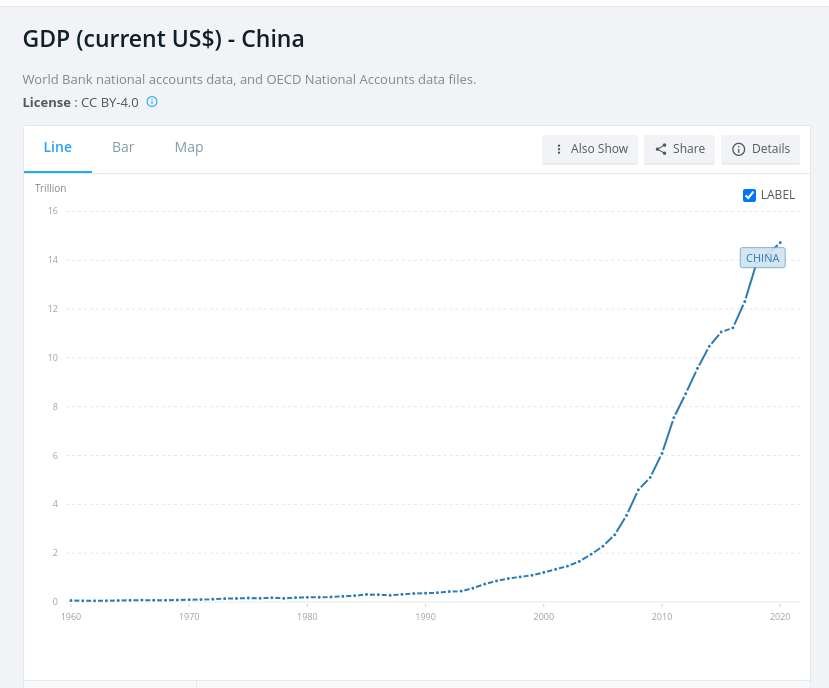
\includegraphics{images/2021-11-25_13-05.png}

Filter China

How to plot ?

\hypertarget{wide-vs-long}{%
\subsubsection{Wide vs long}\label{wide-vs-long}}

\includegraphics{https://tavareshugo.github.io/r-intro-tidyverse-gapminder/fig/07-data_shapes.png}

\begin{itemize}
\item
  Wide data is for humans
\item
  Long data is for computers
\end{itemize}

\includegraphics{https://www.fromthebottomoftheheap.net/assets/img/posts/tidyr-longer-wider.gif}

\hypertarget{wide-to-long}{%
\paragraph{Wide to long}\label{wide-to-long}}

gdp

\begin{Shaded}
\begin{Highlighting}[]
\NormalTok{gap\_wide }\SpecialCharTok{\%\textgreater{}\%} 
  \FunctionTok{select}\NormalTok{(continent}\SpecialCharTok{:}\NormalTok{gdpPercap\_2007) }\SpecialCharTok{\%\textgreater{}\%} 
  \FunctionTok{pivot\_longer}\NormalTok{(}\AttributeTok{cols =}\NormalTok{ gdpPercap\_1952}\SpecialCharTok{:}\NormalTok{gdpPercap\_2007, }
               \AttributeTok{names\_to =} \StringTok{"gdp\_year"}\NormalTok{, }
               \AttributeTok{values\_to =} \StringTok{"gdp\_value"}\NormalTok{) }\SpecialCharTok{\%\textgreater{}\%} 
  \FunctionTok{filter}\NormalTok{(country }\SpecialCharTok{==} \StringTok{"China"}\NormalTok{) }\SpecialCharTok{\%\textgreater{}\%} 
  \FunctionTok{ggplot}\NormalTok{(}\FunctionTok{aes}\NormalTok{(}\AttributeTok{x =}\NormalTok{ gdp\_year, }
             \AttributeTok{y =}\NormalTok{ gdp\_value, }
             \AttributeTok{group =}\NormalTok{ country)) }\SpecialCharTok{+} 
  \FunctionTok{geom\_line}\NormalTok{()}
\end{Highlighting}
\end{Shaded}

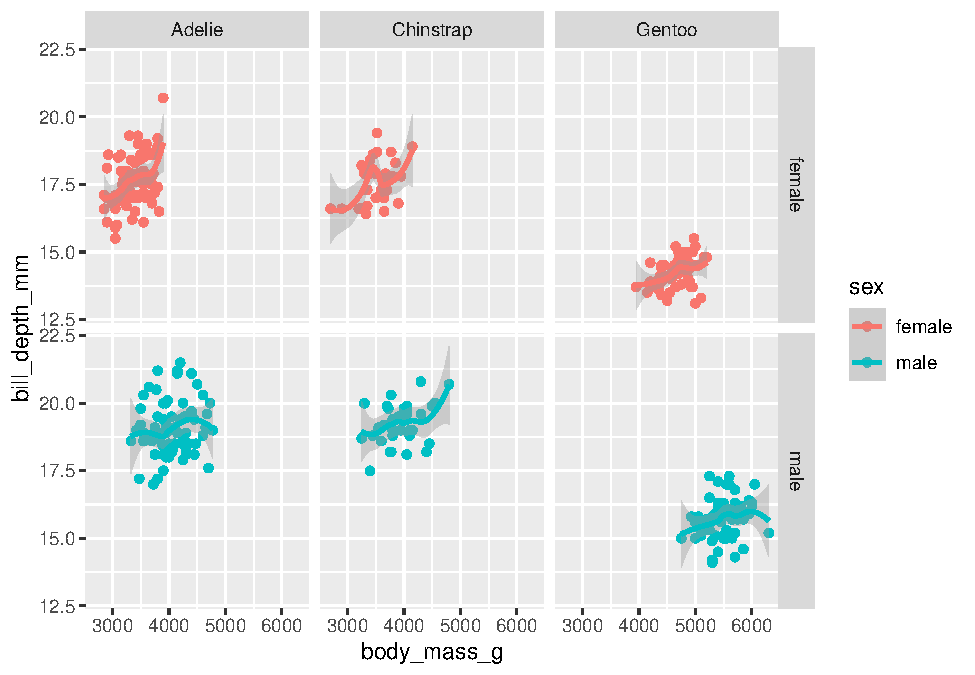
\includegraphics{04_2021_mastering_your_data_files/figure-latex/unnamed-chunk-14-1.pdf}

try to plot

Filter only China

Conects the points

Filter Europe and conects the points

\hypertarget{split-apply-combine}{%
\subsection{Split-apply-combine}\label{split-apply-combine}}

\includegraphics{https://camo.githubusercontent.com/e88a57d67827311f6015cae7f15557052ec44adf5924f83f6d90c62c66be191c/687474703a2f2f7777772e686f66726f652e6e65742f737461743537392f736c696465732f73706c69742d6170706c792d636f6d62696e652e706e67}

Now, we will use the long gapminder dataset

\hypertarget{question-how-has-gdp-per-continent-evolved-per-year}{%
\subsubsection{Question: how has GDP per continent evolved per
year?}\label{question-how-has-gdp-per-continent-evolved-per-year}}

\begin{Shaded}
\begin{Highlighting}[]
\NormalTok{gapminder }\SpecialCharTok{\%\textgreater{}\%} 
  \FunctionTok{filter}\NormalTok{(year }\SpecialCharTok{==} \DecValTok{2007}\NormalTok{) }\SpecialCharTok{\%\textgreater{}\%} 
  \FunctionTok{group\_by}\NormalTok{(continent) }\SpecialCharTok{\%\textgreater{}\%} 
  \FunctionTok{summarise}\NormalTok{(}\AttributeTok{mean\_gdp =} \FunctionTok{mean}\NormalTok{(gdpPercap), }
            \AttributeTok{mean\_pop =} \FunctionTok{mean}\NormalTok{(pop), }
            \AttributeTok{mean\_lifeexp =} \FunctionTok{mean}\NormalTok{(lifeExp), }
            \AttributeTok{n =} \FunctionTok{n}\NormalTok{())}
\end{Highlighting}
\end{Shaded}

\begin{verbatim}
## # A tibble: 5 x 5
##   continent mean_gdp   mean_pop mean_lifeexp     n
##   <fct>        <dbl>      <dbl>        <dbl> <int>
## 1 Africa       3089.  17875763.         54.8    52
## 2 Americas    11003.  35954847.         73.6    25
## 3 Asia        12473. 115513752.         70.7    33
## 4 Europe      25054.  19536618.         77.6    30
## 5 Oceania     29810.  12274974.         80.7     2
\end{verbatim}

\begin{Shaded}
\begin{Highlighting}[]
\NormalTok{gapminder }\SpecialCharTok{\%\textgreater{}\%} 
  \FunctionTok{group\_by}\NormalTok{(continent, year) }\SpecialCharTok{\%\textgreater{}\%} 
  \FunctionTok{summarise}\NormalTok{(}\AttributeTok{gdp\_mean =} \FunctionTok{mean}\NormalTok{(gdpPercap)) }\SpecialCharTok{\%\textgreater{}\%} 
  \FunctionTok{ggplot}\NormalTok{(}\FunctionTok{aes}\NormalTok{(}\AttributeTok{x =}\NormalTok{ year, }
             \AttributeTok{y =}\NormalTok{ gdp\_mean, }
             \AttributeTok{color =}\NormalTok{ continent)) }\SpecialCharTok{+} 
  \FunctionTok{geom\_line}\NormalTok{() }\SpecialCharTok{+} 
  \FunctionTok{scale\_y\_log10}\NormalTok{()}
\end{Highlighting}
\end{Shaded}

\begin{verbatim}
## `summarise()` has grouped output by 'continent'. You can override using the `.groups` argument.
\end{verbatim}

\includegraphics{04_2021_mastering_your_data_files/figure-latex/unnamed-chunk-20-1.pdf}

\hypertarget{question-how-has-population-per-continent-evolved-per-year}{%
\subsubsection{Question: how has POPULATION per continent evolved per
year?}\label{question-how-has-population-per-continent-evolved-per-year}}

Hint: Try log10

\hypertarget{example-vaccinations-latvia}{%
\subsection{Example: Vaccinations
Latvia}\label{example-vaccinations-latvia}}

Homework: See
\href{https://github.com/owid/covid-19-data/tree/master/public/data/vaccinations}{\textless https://github.com/owid/covid-19-data/tree/master/public/data/vaccinations\textgreater{}}

\begin{Shaded}
\begin{Highlighting}[]
\NormalTok{covid\_vac }\OtherTok{\textless{}{-}} \FunctionTok{read\_csv}\NormalTok{(}\StringTok{"https://github.com/owid/covid{-}19{-}data/raw/master/public/data/vaccinations/vaccinations.csv"}\NormalTok{)}
\end{Highlighting}
\end{Shaded}

\begin{verbatim}
## Rows: 63861 Columns: 16
\end{verbatim}

\begin{verbatim}
## -- Column specification --------------------------------------------------------
## Delimiter: ","
## chr   (2): location, iso_code
## dbl  (13): total_vaccinations, people_vaccinated, people_fully_vaccinated, t...
## date  (1): date
\end{verbatim}

\begin{verbatim}
## 
## i Use `spec()` to retrieve the full column specification for this data.
## i Specify the column types or set `show_col_types = FALSE` to quiet this message.
\end{verbatim}

\begin{Shaded}
\begin{Highlighting}[]
\NormalTok{covid\_vac }\SpecialCharTok{\%\textgreater{}\%} 
  \FunctionTok{filter}\NormalTok{(location }\SpecialCharTok{==} \StringTok{"Latvia"}\NormalTok{) }\SpecialCharTok{\%\textgreater{}\%} 
  \FunctionTok{ggplot}\NormalTok{(}\FunctionTok{aes}\NormalTok{(}\AttributeTok{x =}\NormalTok{ date, }
             \AttributeTok{y =}\NormalTok{ total\_vaccinations)) }\SpecialCharTok{+} 
  \FunctionTok{geom\_point}\NormalTok{() }
\end{Highlighting}
\end{Shaded}

\begin{verbatim}
## Warning: Removed 10 rows containing missing values (geom_point).
\end{verbatim}

\includegraphics{04_2021_mastering_your_data_files/figure-latex/unnamed-chunk-22-1.pdf}

\end{document}
